% Options for packages loaded elsewhere
\PassOptionsToPackage{unicode}{hyperref}
\PassOptionsToPackage{hyphens}{url}
%
\documentclass[
]{book}
\title{Biorplot Documentation}
\author{Zheng Hu}
\date{2022-03-16}

\usepackage{amsmath,amssymb}
\usepackage{lmodern}
\usepackage{iftex}
\ifPDFTeX
  \usepackage[T1]{fontenc}
  \usepackage[utf8]{inputenc}
  \usepackage{textcomp} % provide euro and other symbols
\else % if luatex or xetex
  \usepackage{unicode-math}
  \defaultfontfeatures{Scale=MatchLowercase}
  \defaultfontfeatures[\rmfamily]{Ligatures=TeX,Scale=1}
\fi
% Use upquote if available, for straight quotes in verbatim environments
\IfFileExists{upquote.sty}{\usepackage{upquote}}{}
\IfFileExists{microtype.sty}{% use microtype if available
  \usepackage[]{microtype}
  \UseMicrotypeSet[protrusion]{basicmath} % disable protrusion for tt fonts
}{}
\makeatletter
\@ifundefined{KOMAClassName}{% if non-KOMA class
  \IfFileExists{parskip.sty}{%
    \usepackage{parskip}
  }{% else
    \setlength{\parindent}{0pt}
    \setlength{\parskip}{6pt plus 2pt minus 1pt}}
}{% if KOMA class
  \KOMAoptions{parskip=half}}
\makeatother
\usepackage{xcolor}
\IfFileExists{xurl.sty}{\usepackage{xurl}}{} % add URL line breaks if available
\IfFileExists{bookmark.sty}{\usepackage{bookmark}}{\usepackage{hyperref}}
\hypersetup{
  pdftitle={Biorplot Documentation},
  pdfauthor={Zheng Hu},
  hidelinks,
  pdfcreator={LaTeX via pandoc}}
\urlstyle{same} % disable monospaced font for URLs
\usepackage{color}
\usepackage{fancyvrb}
\newcommand{\VerbBar}{|}
\newcommand{\VERB}{\Verb[commandchars=\\\{\}]}
\DefineVerbatimEnvironment{Highlighting}{Verbatim}{commandchars=\\\{\}}
% Add ',fontsize=\small' for more characters per line
\usepackage{framed}
\definecolor{shadecolor}{RGB}{248,248,248}
\newenvironment{Shaded}{\begin{snugshade}}{\end{snugshade}}
\newcommand{\AlertTok}[1]{\textcolor[rgb]{0.94,0.16,0.16}{#1}}
\newcommand{\AnnotationTok}[1]{\textcolor[rgb]{0.56,0.35,0.01}{\textbf{\textit{#1}}}}
\newcommand{\AttributeTok}[1]{\textcolor[rgb]{0.77,0.63,0.00}{#1}}
\newcommand{\BaseNTok}[1]{\textcolor[rgb]{0.00,0.00,0.81}{#1}}
\newcommand{\BuiltInTok}[1]{#1}
\newcommand{\CharTok}[1]{\textcolor[rgb]{0.31,0.60,0.02}{#1}}
\newcommand{\CommentTok}[1]{\textcolor[rgb]{0.56,0.35,0.01}{\textit{#1}}}
\newcommand{\CommentVarTok}[1]{\textcolor[rgb]{0.56,0.35,0.01}{\textbf{\textit{#1}}}}
\newcommand{\ConstantTok}[1]{\textcolor[rgb]{0.00,0.00,0.00}{#1}}
\newcommand{\ControlFlowTok}[1]{\textcolor[rgb]{0.13,0.29,0.53}{\textbf{#1}}}
\newcommand{\DataTypeTok}[1]{\textcolor[rgb]{0.13,0.29,0.53}{#1}}
\newcommand{\DecValTok}[1]{\textcolor[rgb]{0.00,0.00,0.81}{#1}}
\newcommand{\DocumentationTok}[1]{\textcolor[rgb]{0.56,0.35,0.01}{\textbf{\textit{#1}}}}
\newcommand{\ErrorTok}[1]{\textcolor[rgb]{0.64,0.00,0.00}{\textbf{#1}}}
\newcommand{\ExtensionTok}[1]{#1}
\newcommand{\FloatTok}[1]{\textcolor[rgb]{0.00,0.00,0.81}{#1}}
\newcommand{\FunctionTok}[1]{\textcolor[rgb]{0.00,0.00,0.00}{#1}}
\newcommand{\ImportTok}[1]{#1}
\newcommand{\InformationTok}[1]{\textcolor[rgb]{0.56,0.35,0.01}{\textbf{\textit{#1}}}}
\newcommand{\KeywordTok}[1]{\textcolor[rgb]{0.13,0.29,0.53}{\textbf{#1}}}
\newcommand{\NormalTok}[1]{#1}
\newcommand{\OperatorTok}[1]{\textcolor[rgb]{0.81,0.36,0.00}{\textbf{#1}}}
\newcommand{\OtherTok}[1]{\textcolor[rgb]{0.56,0.35,0.01}{#1}}
\newcommand{\PreprocessorTok}[1]{\textcolor[rgb]{0.56,0.35,0.01}{\textit{#1}}}
\newcommand{\RegionMarkerTok}[1]{#1}
\newcommand{\SpecialCharTok}[1]{\textcolor[rgb]{0.00,0.00,0.00}{#1}}
\newcommand{\SpecialStringTok}[1]{\textcolor[rgb]{0.31,0.60,0.02}{#1}}
\newcommand{\StringTok}[1]{\textcolor[rgb]{0.31,0.60,0.02}{#1}}
\newcommand{\VariableTok}[1]{\textcolor[rgb]{0.00,0.00,0.00}{#1}}
\newcommand{\VerbatimStringTok}[1]{\textcolor[rgb]{0.31,0.60,0.02}{#1}}
\newcommand{\WarningTok}[1]{\textcolor[rgb]{0.56,0.35,0.01}{\textbf{\textit{#1}}}}
\usepackage{longtable,booktabs,array}
\usepackage{calc} % for calculating minipage widths
% Correct order of tables after \paragraph or \subparagraph
\usepackage{etoolbox}
\makeatletter
\patchcmd\longtable{\par}{\if@noskipsec\mbox{}\fi\par}{}{}
\makeatother
% Allow footnotes in longtable head/foot
\IfFileExists{footnotehyper.sty}{\usepackage{footnotehyper}}{\usepackage{footnote}}
\makesavenoteenv{longtable}
\usepackage{graphicx}
\makeatletter
\def\maxwidth{\ifdim\Gin@nat@width>\linewidth\linewidth\else\Gin@nat@width\fi}
\def\maxheight{\ifdim\Gin@nat@height>\textheight\textheight\else\Gin@nat@height\fi}
\makeatother
% Scale images if necessary, so that they will not overflow the page
% margins by default, and it is still possible to overwrite the defaults
% using explicit options in \includegraphics[width, height, ...]{}
\setkeys{Gin}{width=\maxwidth,height=\maxheight,keepaspectratio}
% Set default figure placement to htbp
\makeatletter
\def\fps@figure{htbp}
\makeatother
\setlength{\emergencystretch}{3em} % prevent overfull lines
\providecommand{\tightlist}{%
  \setlength{\itemsep}{0pt}\setlength{\parskip}{0pt}}
\setcounter{secnumdepth}{5}
\usepackage{booktabs}
\ifLuaTeX
  \usepackage{selnolig}  % disable illegal ligatures
\fi
\usepackage[]{natbib}
\bibliographystyle{plainnat}

\begin{document}
\maketitle

{
\setcounter{tocdepth}{1}
\tableofcontents
}
\hypertarget{installation-usage}{%
\chapter{Installation \& Usage}\label{installation-usage}}

TODO

\hypertarget{dependence}{%
\section{Dependence}\label{dependence}}

\hypertarget{example}{%
\section{example}\label{example}}

\hypertarget{basic-plot}{%
\chapter{Basic Plot}\label{basic-plot}}

Some basic plots commonly used

\hypertarget{bior_sankey}{%
\section{Bior\_Sankey}\label{bior_sankey}}

\textbf{Description}\\
A sankey plot, you can use Nodes.colour and Nodes.order to set Nodes colour and
order, this function will automatically remove links\$value==0 rows\\
\textbf{Usage}\\
Bior\_Sankey(links, Nodes.colour=NULL, Nodes.order=NULL, fontSize=12,nodeWidth=30,
nodePadding=10, margin=NULL, height=600, width=600, sinksRight=TRUE)\\
\textbf{Arguments}\\
* links: A dataframe, colnames must have `source' `target' `value'\\
* Nodes.colour: Set nodes colour\\
* Nodes.order: Set nodes order\\
* fontSize: Set fontsize\\
* nodeWidth: Set nodewidth\\
* nodePadding: Set the gap size between nodes\\
* margin: R margin\\
* height: numeric height for the network graph's frame area in pixels\\
* width: numeric width for the network graph's frame area in pixels\\
* sinksRight: boolean. If TRUE, the last nodes are moved to the right border of the plot\\
\textbf{Examples}\\

\begin{Shaded}
\begin{Highlighting}[]
\CommentTok{\# links data, colnames must have \textquotesingle{}source\textquotesingle{} \textquotesingle{}target\textquotesingle{} \textquotesingle{}value\textquotesingle{}}
\NormalTok{links }\OtherTok{\textless{}{-}} \FunctionTok{data.frame}\NormalTok{(}
  \AttributeTok{source=}\FunctionTok{c}\NormalTok{(}\StringTok{"C"}\NormalTok{,}\StringTok{"A"}\NormalTok{, }\StringTok{"B"}\NormalTok{, }\StringTok{"E"}\NormalTok{, }\StringTok{"D"}\NormalTok{), }
  \AttributeTok{target=}\FunctionTok{c}\NormalTok{(}\StringTok{"b"}\NormalTok{,}\StringTok{"c"}\NormalTok{, }\StringTok{"a"}\NormalTok{, }\StringTok{"e"}\NormalTok{, }\StringTok{"d"}\NormalTok{), }
  \AttributeTok{value=}\FunctionTok{c}\NormalTok{(}\DecValTok{1}\NormalTok{, }\DecValTok{2}\NormalTok{, }\DecValTok{0}\NormalTok{, }\DecValTok{4}\NormalTok{, }\DecValTok{5}\NormalTok{)}
\NormalTok{)}
\CommentTok{\# Set Nodes order and colour}
\NormalTok{Nodes.order }\OtherTok{\textless{}{-}} \FunctionTok{c}\NormalTok{(}\StringTok{"A"}\NormalTok{, }\StringTok{"B"}\NormalTok{, }\StringTok{"C"}\NormalTok{, }\StringTok{"D"}\NormalTok{, }\StringTok{"E"}\NormalTok{, }\StringTok{"a"}\NormalTok{, }\StringTok{"b"}\NormalTok{, }\StringTok{"c"}\NormalTok{, }\StringTok{"d"}\NormalTok{, }\StringTok{"e"}\NormalTok{)}
\NormalTok{Nodes.colour }\OtherTok{\textless{}{-}} \FunctionTok{pal\_d3}\NormalTok{(}\StringTok{"category20"}\NormalTok{, }\AttributeTok{alpha =} \FloatTok{0.7}\NormalTok{)(}\DecValTok{20}\NormalTok{)}
\NormalTok{p }\OtherTok{\textless{}{-}} \FunctionTok{Bior\_Sankey}\NormalTok{(links, }\AttributeTok{Nodes.order=}\NormalTok{Nodes.order, }\AttributeTok{Nodes.colour=}\NormalTok{Nodes.colour, }\AttributeTok{fontSize=}\DecValTok{20}\NormalTok{)}
\NormalTok{p}
\CommentTok{\# Use saveNetwork() to save the plot as html}
\FunctionTok{saveNetwork}\NormalTok{(p,}\StringTok{"sankey.html"}\NormalTok{)}
\end{Highlighting}
\end{Shaded}

\begin{verbatim}
    <iframe allowtransparency="yes" frameborder="0" width="300" height="300" src="images/sankey.html"/>
</div>
\end{verbatim}

\hypertarget{bior_pie}{%
\section{Bior\_pie}\label{bior_pie}}

\textbf{Description}\\
Pie plot\\
\textbf{Usage}\\
Bior\_pie(x, labels, col=pal\_d3(``category20'',alpha=0.7)(20), title=``\,``, fontsize=20, legend.key.size=1)\\
\textbf{Arguments}\\
* x: A vector of value\\
* labels: A vector of labels for x\\
* col: colour\\
* title: title\\
* fontsize: fontsize\\
* legend.key.size: legend size\\
\textbf{Examples}\\

\begin{Shaded}
\begin{Highlighting}[]
\NormalTok{x }\OtherTok{\textless{}{-}} \FunctionTok{c}\NormalTok{(}\DecValTok{3}\NormalTok{,}\DecValTok{7}\NormalTok{,}\DecValTok{9}\NormalTok{,}\DecValTok{1}\NormalTok{,}\DecValTok{2}\NormalTok{)}
\NormalTok{labels }\OtherTok{\textless{}{-}} \FunctionTok{c}\NormalTok{(}\StringTok{"A"}\NormalTok{, }\StringTok{"B"}\NormalTok{, }\StringTok{"C"}\NormalTok{, }\StringTok{"D"}\NormalTok{, }\StringTok{"E"}\NormalTok{)}
\NormalTok{col }\OtherTok{\textless{}{-}} \FunctionTok{c}\NormalTok{(}\StringTok{"\#AEC7E8B2"}\NormalTok{, }\StringTok{"\#FFBB78B2"}\NormalTok{, }\StringTok{"\#98DF8AB2"}\NormalTok{, }\StringTok{"\#FF9896B2"}\NormalTok{, }\StringTok{"\#C5B0D5B2"}\NormalTok{)}
\NormalTok{p }\OtherTok{\textless{}{-}} \FunctionTok{Bior\_pie}\NormalTok{(x, labels, }\AttributeTok{col=}\NormalTok{col, }\AttributeTok{title=}\StringTok{"Test Bior\_pie"}\NormalTok{)}
\NormalTok{p}
\end{Highlighting}
\end{Shaded}

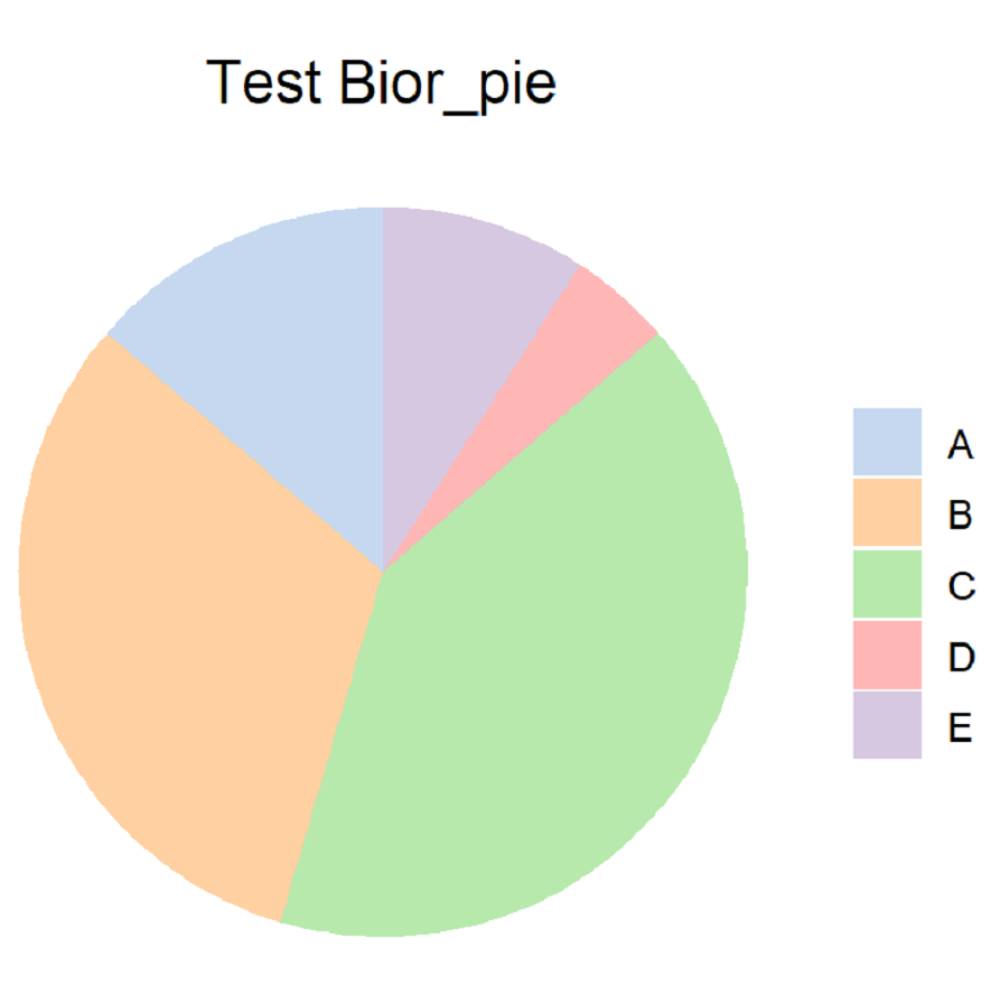
\includegraphics{images/Bior_pie.png}

\hypertarget{scrnaseq-plot}{%
\chapter{scRNAseq Plot}\label{scrnaseq-plot}}

Some plots commonly used in scRNAseq analysis.\\
The test data used in Examples is \href{https://satijalab.org/seurat/archive/v3.1/pbmc3k_tutorial.html}{Seurat Tutorial Data}\\

\begin{Shaded}
\begin{Highlighting}[]
\CommentTok{\# load test data}
\NormalTok{seuratobject }\OtherTok{\textless{}{-}} \FunctionTok{readRDS}\NormalTok{(}\StringTok{"testdata/pbmc3k\_final.rds"}\NormalTok{)}
\CommentTok{\# colors}
\NormalTok{cols }\OtherTok{\textless{}{-}} \FunctionTok{pal\_d3}\NormalTok{(}\StringTok{"category20"}\NormalTok{)(}\DecValTok{20}\NormalTok{)}
\end{Highlighting}
\end{Shaded}

\hypertarget{bior_dimplot}{%
\section{Bior\_DimPlot}\label{bior_dimplot}}

\textbf{Description}\\
Plot based on Seurat::DimPlot()\\
\textbf{Usage}\\
Bior\_DimPlot(seuratobject, reduction=``umap'', pt.size=1, label = TRUE, label.size=5, cols=NULL)\\
\textbf{Arguments}\\
* seuratobject: Seurat object\\
* reduction: Choose ``umap'' or ``tsne''\\
* pt.size: Adjust cell point size\\
* label: Whether to label the clusters\\
* label.size: Sets size of labels\\
* cols: colors\\
\textbf{Examples}

\begin{Shaded}
\begin{Highlighting}[]
\NormalTok{p }\OtherTok{\textless{}{-}} \FunctionTok{Bior\_DimPlot}\NormalTok{(seuratobject, }\AttributeTok{cols =}\NormalTok{ cols)}
\NormalTok{p}
\end{Highlighting}
\end{Shaded}

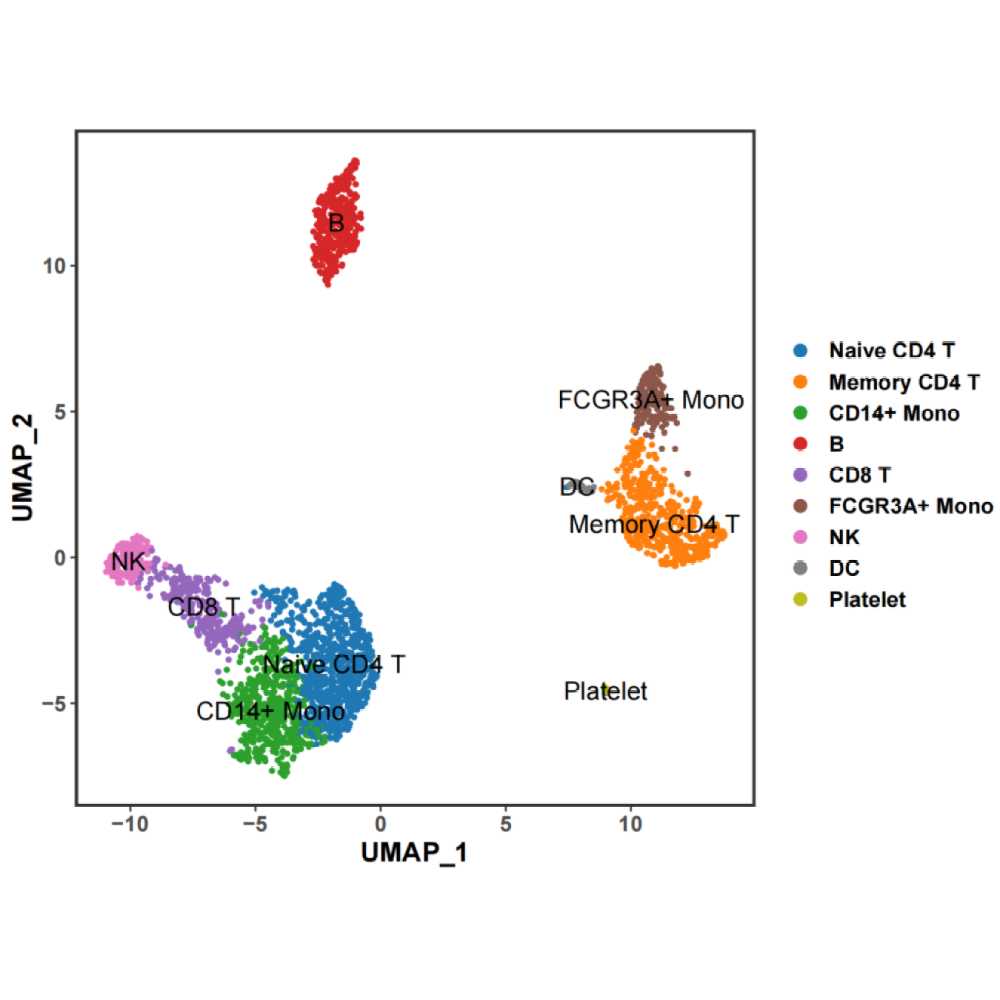
\includegraphics{images/Bior_DimPlot.png}

\hypertarget{bior_featurevlnplot}{%
\section{Bior\_FeatureVlnplot}\label{bior_featurevlnplot}}

\textbf{Description}\\
Simultaneously plot multiple genes Featureplot and Vlnplot\\
\textbf{Usage}\\
Bior\_FeatureVlnplot(seuratobject, genes, title.size=15, axis.text.size=10, pt.size=1, nrow=1, scale=1, cols=NULL)\\
\textbf{Arguments}\\
* seuratobject: Seurat object\\
* genes: Multiple genes vectors, eg: c(``MS4A1'', ``GNLY'', ``CD3E'')\\
* title.size: title gene name size\\
* axis.text.size: x-axis text size\\
* pt.size: Featureplot point size\\
* nrow: Number of rows in the plot grid\\
* scale: scale the size of all or select plots\\
* cols: Vlnplot cluster colors\\
\textbf{Examples}\\

\begin{Shaded}
\begin{Highlighting}[]
\NormalTok{genes }\OtherTok{\textless{}{-}} \FunctionTok{c}\NormalTok{(}\StringTok{"MS4A1"}\NormalTok{, }\StringTok{"GNLY"}\NormalTok{, }\StringTok{"CD3E"}\NormalTok{, }\StringTok{"CD14"}\NormalTok{, }\StringTok{"FCER1A"}\NormalTok{, }\StringTok{"FCGR3A"}\NormalTok{)}
\NormalTok{p }\OtherTok{\textless{}{-}} \FunctionTok{Bior\_FeatureVlnplot}\NormalTok{(seuratobject, genes, }\AttributeTok{scale=}\FloatTok{0.8}\NormalTok{, }\AttributeTok{pt.size=}\FloatTok{0.5}\NormalTok{, }\AttributeTok{nrow=}\DecValTok{2}\NormalTok{, }\AttributeTok{cols=}\NormalTok{cols)}
\NormalTok{p}
\end{Highlighting}
\end{Shaded}

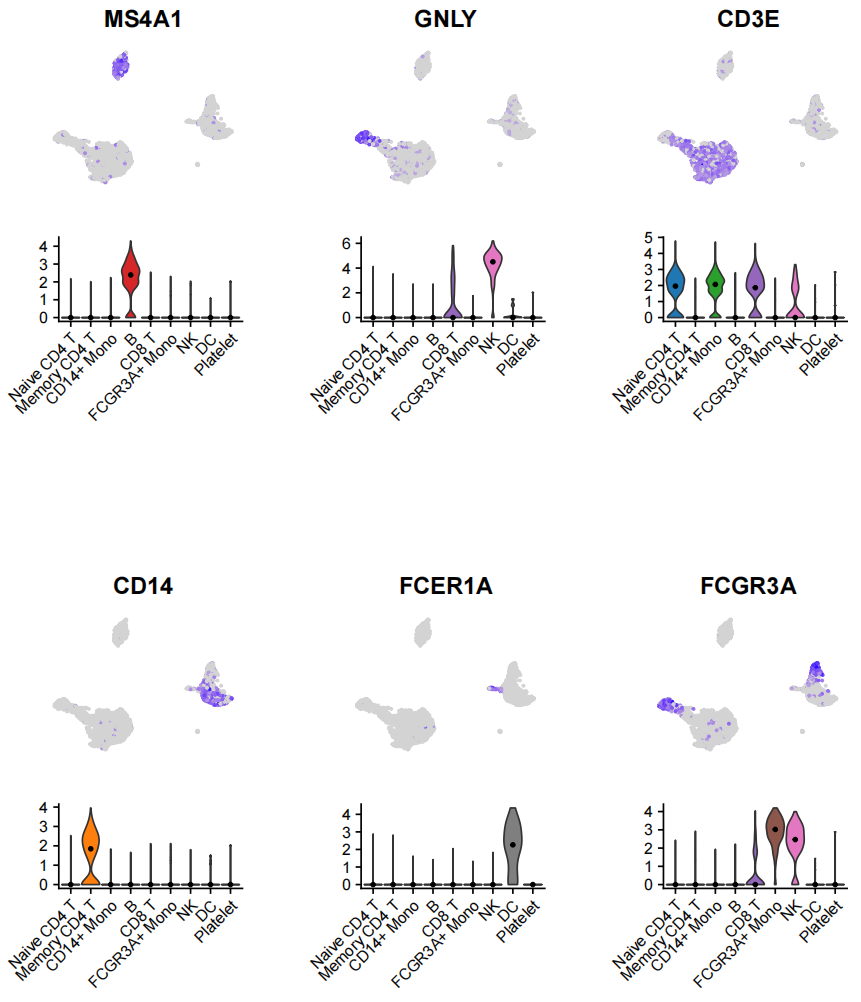
\includegraphics{images/Bior_FeatureVlnplot.png}

\hypertarget{ngs-plot}{%
\chapter{NGS Plot}\label{ngs-plot}}

  \bibliography{book.bib,packages.bib}

\end{document}
